\documentclass[a4paper]{article}

\usepackage{listings}
\usepackage{color}
\usepackage{graphicx}
\usepackage{tikz}
\usepackage{multicol}

\usepackage[top=2.0cm, bottom=2.0cm, left=2.0cm, right=2.0cm]{geometry}

\begin{document}

\title{Embbeded Systems - Exercise 03}

\author{Jander Nascimento}

\maketitle

\section*{Question 1}

Give initial predicate and transition predicate.

Initial predicate $v_1(var1),v_2(var2)$:

$I(v_1,v_2)=\neg v_1 \land \neg v_2 $

Transition predicate $v_1(var1),v_2(var2),v_1'(var1'),v_2'(var2')$:

$\exists f_1,f_2.\newline 
(f_1 \rightarrow (v_1 \leftrightarrow \neg v_1')) \land (\neg f_1 \rightarrow (v_1 \leftrightarrow v_1')) \newline
(f_2 \rightarrow (v_2 \leftrightarrow \neg v_2')) \land (\neg f_2 \rightarrow (v_2 \leftrightarrow v_2'))
$

Combining the possibilities:

$
((v_1 \leftrightarrow \neg v_1') \land (v_2 \leftrightarrow \neg v_2')) \lor \newline
((v_1 \leftrightarrow \neg v_1') \land (v_2 \leftrightarrow v_2')) \lor \newline
((v_1 \leftrightarrow v_1') \land (v_2 \leftrightarrow \neg v_2')) \lor \newline
((v_1 \leftrightarrow v_1') \land (v_2 \leftrightarrow v_2')) \newline
$




\section*{Question 2}

\begin{multicols}{4}

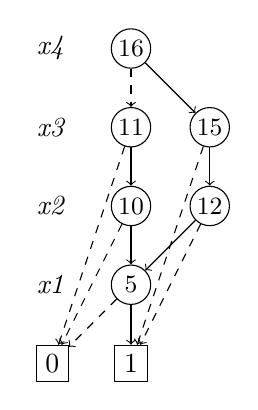
\begin{tikzpicture}[node distance=1cm]
  \tikzstyle{BDDnode}=[circle,draw=black,inner sep=0pt,minimum size=5mm]
  \node[] (vx4) {$\mathit{x4}$};
  \node[xshift=0cm, BDDnode, right of=vx4] (n16) {\small $16$};

  \node[below of=vx4] (vx3) {$\mathit{x3}$};
  \node[xshift=0cm, BDDnode, right of=vx3] (n11) {\small $11$};
  \node[xshift=0cm, BDDnode, right of=n11] (n15) {\small $15$};

  \node[below of=vx3] (vx2) {$\mathit{x2}$};
  \node[xshift=0cm, BDDnode, right of=vx2] (n10) {\small $10$};
  \node[xshift=0cm, BDDnode, right of=n10] (n12) {\small $12$};

  \node[below of=vx2] (vx1) {$\mathit{x1}$};
  \node[xshift=0cm, BDDnode, right of=vx1] (n5) {\small $5$};


  % terminals
  \node[draw=black, style=rectangle, below of=vx1, xshift=1cm] (n1) {$1$};
  \node[draw=black, style=rectangle, left of=n1] (n0) {$0$};

  % edges

  \draw[->,dashed] (n5) -> (n0);
  \draw[->] (n5) -> (n1);
  \draw[->,dashed] (n10) -> (n0);
  \draw[->] (n10) -> (n5);
  \draw[->,dashed] (n11) -> (n0);
  \draw[->] (n11) -> (n10);
  \draw[->,dashed] (n12) -> (n1);
  \draw[->] (n12) -> (n5);
  \draw[->,dashed] (n15) -> (n1);
  \draw[->] (n15) -> (n12);
  \draw[->,dashed] (n16) -> (n11);
  \draw[->] (n16) -> (n15);

\end{tikzpicture}

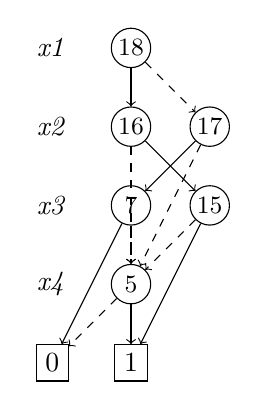
\begin{tikzpicture}[node distance=1cm]
  \tikzstyle{BDDnode}=[circle,draw=black,inner sep=0pt,minimum size=5mm]
  \node[] (vx1) {$\mathit{x1}$};
  \node[xshift=0cm, BDDnode, right of=vx1] (n18) {\small $18$};

  \node[below of=vx1] (vx2) {$\mathit{x2}$};
  \node[xshift=0cm, BDDnode, right of=vx2] (n16) {\small $16$};
  \node[xshift=0cm, BDDnode, right of=n16] (n17) {\small $17$};

  \node[below of=vx2] (vx3) {$\mathit{x3}$};
  \node[xshift=0cm, BDDnode, right of=vx3] (n7) {\small $7$};
  \node[xshift=0cm, BDDnode, right of=n7] (n15) {\small $15$};

  \node[below of=vx3] (vx4) {$\mathit{x4}$};
  \node[xshift=0cm, BDDnode, right of=vx4] (n5) {\small $5$};


  % terminals
  \node[draw=black, style=rectangle, below of=vx4, xshift=1cm] (n1) {$1$};
  \node[draw=black, style=rectangle, left of=n1] (n0) {$0$};

  % edges

  \draw[->,dashed] (n5) -> (n0);
  \draw[->] (n5) -> (n1);
  \draw[->,dashed] (n7) -> (n5);
  \draw[->] (n7) -> (n0);
  \draw[->,dashed] (n15) -> (n5);
  \draw[->] (n15) -> (n1);
  \draw[->,dashed] (n16) -> (n5);
  \draw[->] (n16) -> (n15);
  \draw[->,dashed] (n17) -> (n5);
  \draw[->] (n17) -> (n7);
  \draw[->,dashed] (n18) -> (n17);
  \draw[->] (n18) -> (n16);

\end{tikzpicture}
		

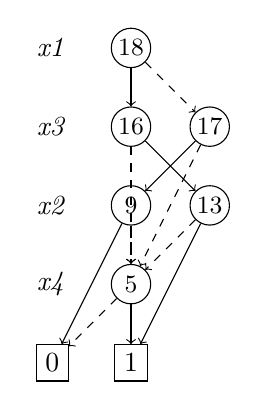
\begin{tikzpicture}[node distance=1cm]
  \tikzstyle{BDDnode}=[circle,draw=black,inner sep=0pt,minimum size=5mm]
  \node[] (vx1) {$\mathit{x1}$};
  \node[xshift=0cm, BDDnode, right of=vx1] (n18) {\small $18$};

  \node[below of=vx1] (vx3) {$\mathit{x3}$};
  \node[xshift=0cm, BDDnode, right of=vx3] (n16) {\small $16$};
  \node[xshift=0cm, BDDnode, right of=n16] (n17) {\small $17$};

  \node[below of=vx3] (vx2) {$\mathit{x2}$};
  \node[xshift=0cm, BDDnode, right of=vx2] (n9) {\small $9$};
  \node[xshift=0cm, BDDnode, right of=n9] (n13) {\small $13$};

  \node[below of=vx2] (vx4) {$\mathit{x4}$};
  \node[xshift=0cm, BDDnode, right of=vx4] (n5) {\small $5$};


  % terminals
  \node[draw=black, style=rectangle, below of=vx4, xshift=1cm] (n1) {$1$};
  \node[draw=black, style=rectangle, left of=n1] (n0) {$0$};

  % edges

  \draw[->,dashed] (n5) -> (n0);
  \draw[->] (n5) -> (n1);
  \draw[->,dashed] (n9) -> (n5);
  \draw[->] (n9) -> (n0);
  \draw[->,dashed] (n13) -> (n5);
  \draw[->] (n13) -> (n1);
  \draw[->,dashed] (n16) -> (n5);
  \draw[->] (n16) -> (n13);
  \draw[->,dashed] (n17) -> (n5);
  \draw[->] (n17) -> (n9);
  \draw[->,dashed] (n18) -> (n17);
  \draw[->] (n18) -> (n16);

\end{tikzpicture}

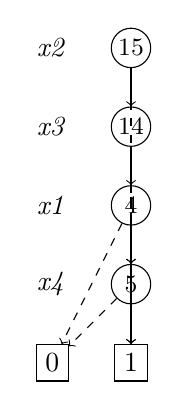
\begin{tikzpicture}[node distance=1cm]
  \tikzstyle{BDDnode}=[circle,draw=black,inner sep=0pt,minimum size=5mm]
  \node[] (vx2) {$\mathit{x2}$};
  \node[xshift=0cm, BDDnode, right of=vx2] (n15) {\small $15$};

  \node[below of=vx2] (vx3) {$\mathit{x3}$};
  \node[xshift=0cm, BDDnode, right of=vx3] (n14) {\small $14$};

  \node[below of=vx3] (vx1) {$\mathit{x1}$};
  \node[xshift=0cm, BDDnode, right of=vx1] (n4) {\small $4$};

  \node[below of=vx1] (vx4) {$\mathit{x4}$};
  \node[xshift=0cm, BDDnode, right of=vx4] (n5) {\small $5$};


  % terminals
  \node[draw=black, style=rectangle, below of=vx4, xshift=1cm] (n1) {$1$};
  \node[draw=black, style=rectangle, left of=n1] (n0) {$0$};

  % edges

  \draw[->,dashed] (n4) -> (n0);
  \draw[->] (n4) -> (n1);
  \draw[->,dashed] (n5) -> (n0);
  \draw[->] (n5) -> (n1);
  \draw[->,dashed] (n14) -> (n5);
  \draw[->] (n14) -> (n4);
  \draw[->,dashed] (n15) -> (n5);
  \draw[->] (n15) -> (n14);

\end{tikzpicture}

\end{multicols}


		Just by looking at the figures, just by changing the order, we influence in the shape of the diagram. The last diagram was created by ordering the elements according to its importance (dependency) in the statement. Thus, more influent variables comes first. 
		
		So the best order would be $ x_2 > x_3 > x_4 \quad or \quad x_1$

\newpage

\section*{Question 3}

	The predicates used to evaluate this was $(out_1 | out_0 | carry) == (x_1 | x_0 | y_1 | y_0)$

	\begin{figure}[h]
			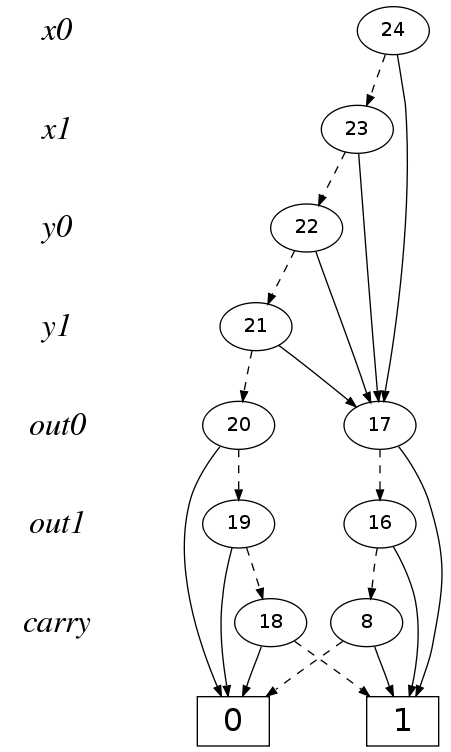
\includegraphics[scale=0.3]{img/q3i1}
	\end{figure}
	
	We can check that the DAG generated is not optimal due to the sequentiality of the initial nodes.

\section*{Question 4}

	MISS

\end{document}
